\documentclass[]{article}
\usepackage{pgfplots}

%opening
\title{How to reach Expert}
\author{Dimael Rivas}

\begin{document}

\maketitle



\section{Context}
This is a kind of blog where I will share how to reach expert. I will follow suggestions from Galen Colin and using an chrome extension I will try to solve at least 1 problem per day. The main idea is to train like an expert.

\section{The plan}
According to Galen Colin, the most "Vital" topics are these:
\begin{itemize}
	\item Dynamic programming
	\item Basic graphs/trees
	\item Number theory - factorization, modular arithmetic, prime factor representation
	\item Basic combinatorics, probability, expected value
	\item Bitwise stuff
	\item Data structures: segment tree, STL (library)
	\item Basics of game theory
	\item Proofs (not a topic, but worth mentioning, greedy)
	\item Constructives
\end{itemize}

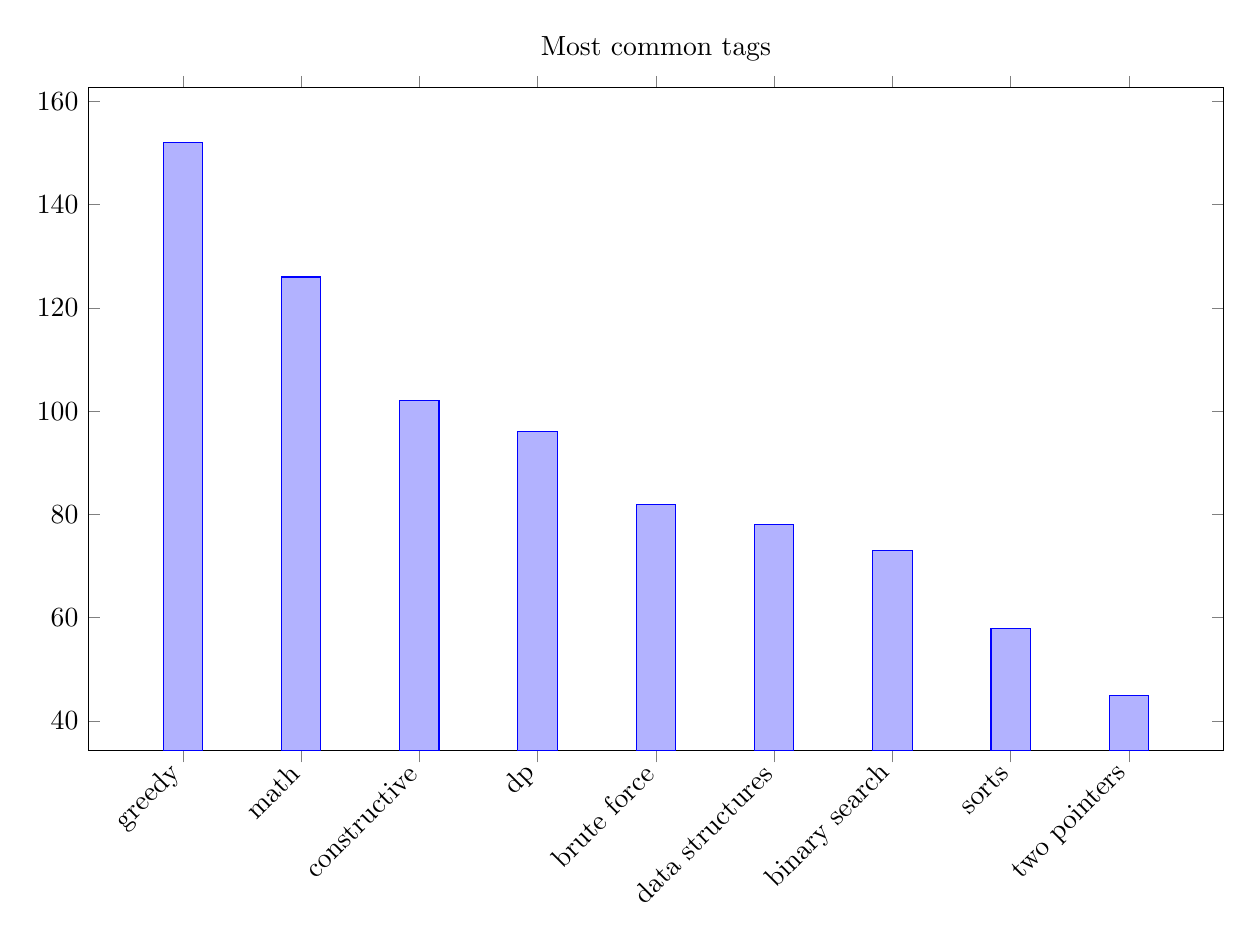
\begin{tikzpicture}
	\begin{axis}
		[
		title=Most common tags,
		ybar,bar width=0.5cm,
		symbolic x coords={greedy,math,constructive,dp,brute force,data structures,binary search,sorts,two pointers},
		width=16cm, % Increased width of the plot
		height=10cm, % Increased height of the plot
		xticklabel style={rotate=45, anchor=east}, % Rotate x-axis labels
		]
		\addplot coordinates{(greedy,152) (math, 126) (constructive, 102) (dp, 96) (brute force, 82) (data structures, 78) (binary search, 73) (sorts, 58) (two pointers, 45)};
	\end{axis}
\end{tikzpicture}

\section{To-do}
Make an script that takes 5 problems with the 5 most common topics
\end{document}
